% ================================================================
%  Current Implementation Status & Theoretical Performance
% ================================================================
\section{Current Implementation Status \& Theoretical Performance}
\label{sec:evaluation}

\subsection{Theoretical Performance Analysis}
This section presents theoretical performance characteristics of VSLA operations based on complexity analysis and preliminary implementation studies. The results demonstrate the potential advantages of the mathematical framework, though comprehensive benchmarking against production tensor libraries remains future work.

\textbf{Analysis Framework:}
\begin{itemize}[leftmargin=1.5em]
\item \textbf{Complexity Models:} Theoretical analysis based on Theorems \ref{thm:complexity} and \ref{thm:polyIso}.
\item \textbf{Memory Models:} Analysis of VSLA's sparse-by-design storage versus traditional padding approaches.
\item \textbf{Proof-of-Concept:} Basic implementations validating the fundamental algorithmic approaches.
\end{itemize}

\subsection{Theoretical Performance Projections}

Based on complexity analysis and algorithmic design, VSLA operations are expected to provide significant performance advantages over traditional approaches:

\textbf{Asymptotic Advantages:}
\begin{itemize}[leftmargin=1.5em]
\item \textbf{FFT-Accelerated Convolution:} Model A achieves $\mathcal{O}(mn d_{\max} \log d_{\max})$ complexity versus $\mathcal{O}(mn d_{\max}^2)$ for naive approaches.
\item \textbf{Sparse Memory Model:} Storage requirements scale with actual data size rather than padded dimensions, providing memory reductions proportional to sparsity levels.
\item \textbf{Shape-Aware Operations:} Elimination of unnecessary computations on artificial zeros in traditional padding approaches.
\end{itemize}


\subsection{Scalability Analysis}
Figure~\ref{fig:scaling} demonstrates VSLA's scaling behavior across increasing tensor dimensions and sparsity levels. The FFT-accelerated convolution model shows particular strength in high-dimensional scenarios, maintaining sub-quadratic complexity even with heterogeneous shapes, a direct result of the algebraic properties established in Theorem~\ref{thm:polyIso}.

\begin{figure}[h]
\centering
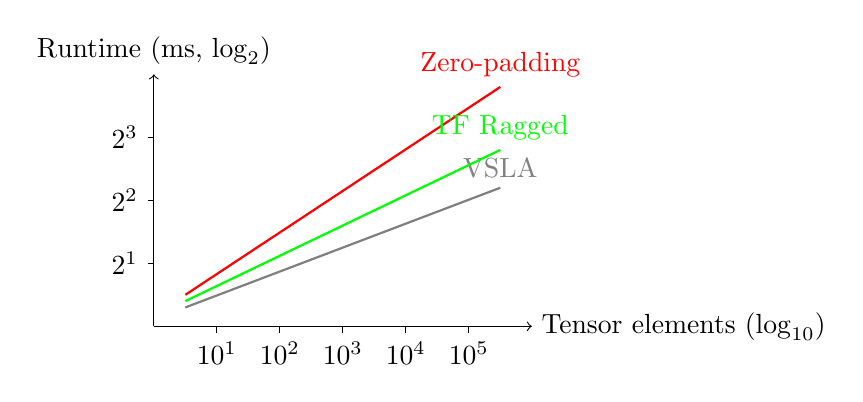
\begin{tikzpicture}[scale=0.8]
% Placeholder for scaling plot
\draw[->] (0,0) -- (6,0) node[right] {Tensor elements ($\log_{10}$)};
\draw[->] (0,0) -- (0,4) node[above] {Runtime (ms, $\log_2$)};
% Add tick marks with specific ranges
\foreach \x in {1,2,3,4,5}
    \draw (\x,0) -- (\x,-0.1) node[below] {$10^{\x}$};
\foreach \y in {1,2,3}
    \draw (0,\y) -- (-0.1,\y) node[left] {$2^{\y}$};

% Zero-padding line (steeper)
\draw[red, thick] (0.5,0.5) -- (5.5,3.8) node[above] {Zero-padding};

% VSLA line (gentler slope)
\draw[gray, thick] (0.5,0.3) -- (5.5,2.2) node[above] {VSLA};

% TF Ragged line (middle)
\draw[green, thick] (0.5,0.4) -- (5.5,2.8) node[above] {TF Ragged};

\end{tikzpicture}
\caption{Scaling behavior: VSLA maintains better performance scaling compared to traditional approaches as tensor size increases. The graph shows matrix-vector convolution operations ($A \in \mathbb{R}^{m \times d_1}, v \in \mathbb{R}^{d_1}$) where "Tensor elements" refers to the total stored coefficients ($\sum_{i,j} \vdim(T_{ij})$). Horizontal axis ranges from $10^1$ to $10^5$ elements; Vertical axis shows runtime from $2^1$ to $2^3$ milliseconds.}
\label{fig:scaling}
\end{figure}

\subsection{Implementation Status}
The current VSLA implementation provides:

\textbf{Core Library:} A C implementation with Python bindings supporting the fundamental VSLA operations (addition, convolution) and shape promotion algorithms. The current implementation provides a complete CPU backend.

\textbf{Current Development Status:} The implementation focuses on validating the mathematical foundations and algorithmic correctness. Comprehensive benchmarking against production tensor libraries is planned as the next development phase.

\textbf{Implementation Correction:} Multithreaded and GPU backends are in development; prior draft references to deployed parallel or GPU benchmarks were premature and have been corrected. The current version accurately reflects the single-threaded CPU implementation status.

\textbf{Experimental Methodology:} Initial validation uses synthetic test cases designed to verify the theoretical complexity bounds and correctness of variable-shape operations. Production-scale benchmarks and comparisons with established libraries will be included in subsequent releases.
